Das OOP Design Pattern \textbf{Adapter} ermöglicht zwei Objekte mit unterschiedlichen Schnittstellen miteinander zu verbinden.
Der Adapter kann übergebene Daten transformieren (z.B. JSON in XML) 
oder die Schnittstelle zweiten Objektes für erstes Objekt anpassen
(z.B. Parameterliste oder Anzahl der Methoden).

\begin{figure}[H]
    \centering
    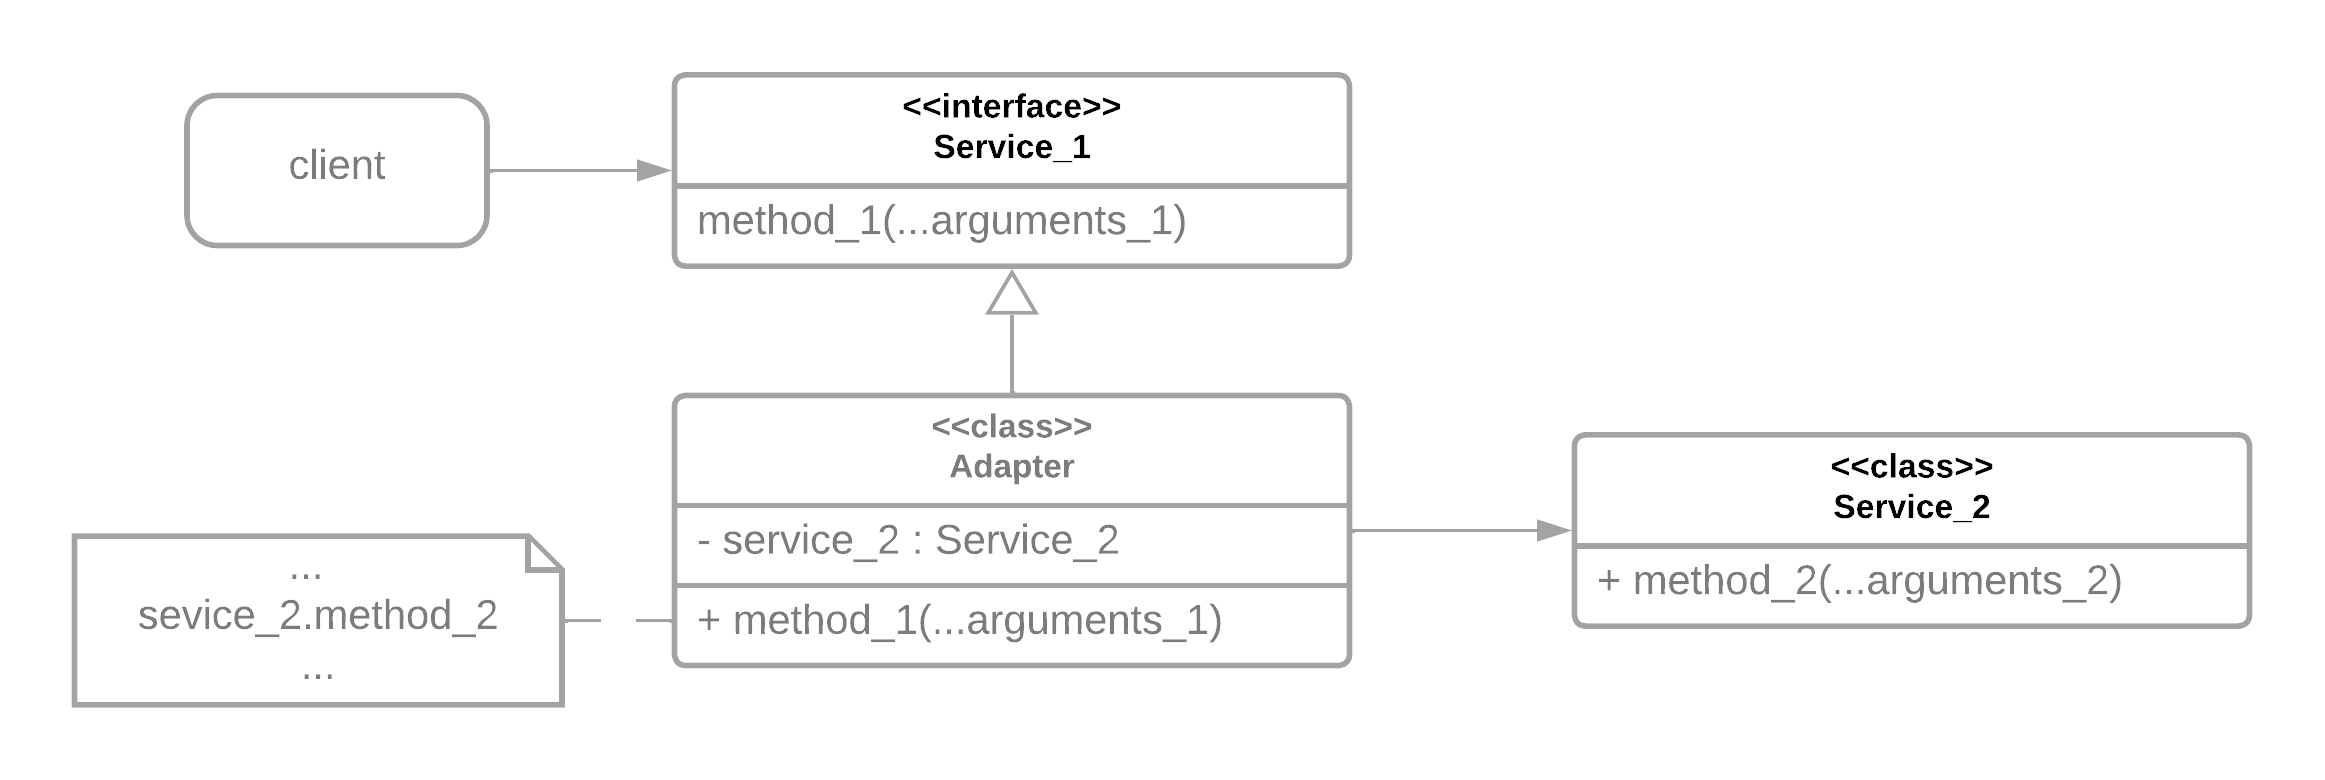
\includegraphics[width=1\textwidth]{Images/OOPAdapter.png}
    \caption[UML Adapter]{Klassendiagrammm Adapter}
    \label{fig:cd_adapter }
\end{figure}